%-------------------------------------------------------------
%-------------------------------------------------------------
%-------------------------------------------------------------
%                          Rozdział 1
%-------------------------------------------------------------
%-------------------------------------------------------------
%-------------------------------------------------------------

\setstretch{1.5}
\setlength{\parindent}{1.25cm} % Ustaw wcięcie akapitu

\section{Opis projektu}

\begin{spacing}{1.5} % Zaczynamy interlinię 1.5
    Projekt zaliczeniowy na ćwiczenia "Przetwarzanie Rozproszone" przedstawia aplikację czat w formie serwerów REST API w C\# i Python oraz klientów w C\#, Python, Powershell.
\end{spacing} % Kończymy interlinię 1.5
\noindent\hspace*{-0.3cm} % Dostosuj wartość -5cm według potrzeb
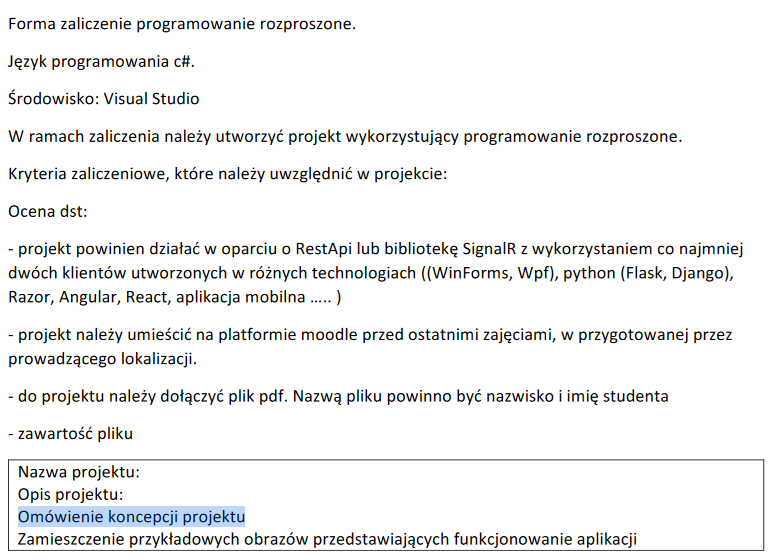
\includegraphics[width=1.0\textwidth]{assets/tekst_zadania.png}
\addcontentsline{lof}{figure}{\protect\numberline{\thefigure}Tekst zadania zaliczeniowego}


\section{Omówienie koncepcji projektu}

\subsection{Wstęp}
\begin{spacing}{1.5} % Zaczynamy interlinię 1.5 
\end{spacing} % Kończymy interlinię 1.5
    Koncepcja przewodząca powyższemu projektowi polega na zaliczeniu przedmiotu Przetwarzanie Rozproszone na ocenę przynajmniej dostateczną. Obrałem technologie Python, Powershell i C\# dlatego, że wymagania wykładowcy obejmują użycie przynajmniej dwóch różnych technologii do utworzenia klienta, a ja wybrałem trzy. Niestety odrzuciłem zakładanie serwera oraz klienta w języku programowania haskell ponieważ ustawianie środowiska dla tego języka programowania może być problematyczne dla wykładowcy skutkując oceną niedostateczną.

\section{Omówienie projektu}
\subsection{Drzewo folderów projektu}
\begin{spacing}{1.5} % Zaczynamy interlinię 1.5
\end{spacing} % Kończymy interlinię 1.5
\begin{table}[ht]
\centering
\caption{Drzewo struktury katalogów}
\label{tab:moja_struktura_katalogow}
        \dirtree{%
        .1 /..
        .2 ApiServerPython\DTcomment{Server napisany w języku programowania Python}.
        .3 ....
        .2 ApiServerC\#\DTcomment{Server napisany w języku programowania C\#}.
        .3 ....
        .3 ....
        .3 ....
        .2 ApiClientC\#\DTcomment{Klient napisany w języku programowania C\#}.
        .3 ....
        .2 ApiClientPowershell\DTcomment{Klient napisany w języku programowania Powershell}.
        .3 ....
        .2 ApiClientPython\DTcomment{Klient napisany w języku programowania Python}.
        .3 ....
        .2 ProjectDocumentation\DTcomment{Dokumentacja projektu zaliczeniowego}.
    }
\end{table}

\subsection{Dlaczego dwa serwery?}
\begin{spacing}{1.5} % Zaczynamy interlinię 1.5
\end{spacing} % Kończymy interlinię 1.5
    Na załączonym powyżej drzewie folderu projektów na pierwszy rzut oka widać, że pomimo jednego wymaganego serwera API REST w języku C\# jest zrobiony dodatkowo serwer API REST w języku Python. Zostało to utworzone ze względu na moje komercyjne doświadczenie w korzystaniu z języka programowania Python. Umożliwiło mi to stworzenie w 100\% działającego serwera, który mogę od razu wykorzystać w celach testowych.

\subsection{Dlaczego trzy klienty?}
\begin{spacing}{1.5} % Zaczynamy interlinię 1.5
    Tak samo jak na powyżej załączonym drzewie folderu projektów widać, że pomimo dwóch wymaganych klientów API REST zrobiony jeden dodatkowy klient. Użyłem języków C\#, Python i Powershell zważywszy na to, że w tych pierwszych dwóch językach są już napisane serwery, a ów trzeci język jest muszlą mocy pozwalającą na niesamowite i błyskawiczne czynności zarówno na środowisku Windows jak i Linux przyćmiewając możliwości oferowane przez powłokę linux.
\end{spacing} % Kończymy interlinię 1.5

\section{Uruchomienie serwerów REST API}

\subsection{Setup i uruchomienie Serwera napisanego w Python}
\begin{spacing}{1.5} % Zaczynamy interlinię 1.5
\end{spacing} % Kończymy interlinię 1.5
    Aby przygotować i uruchomić serwer FastAPI napisany w języku programowania Python manualnie, należy wykonać następujące kroki:
    \begin{enumerate}
        \item Upewnij się, że Python w wersji 3.x. jest zainstalowany w systemie.
        \item Przejdź do katalogu projektu serwera, gdzie znajduje się plik \texttt{.py}:
        \begin{lstlisting}[language=bash]
    cd sciezka/do/projektu/ApiServerPython
        \end{lstlisting}
        \item Zainstaluj potrzebny pakiet \texttt{requests} używając \texttt{pip}:
        \begin{lstlisting}[language=bash]
    pip install fastapi uvicorn pydantic
        \end{lstlisting}
        \item Uruchom serwer używając \texttt{uvicorn}:
        \begin{lstlisting}[language=bash]
        uvicorn api_server:app 
            --host localhost --port 1337 --reload
        \end{lstlisting}
    \end{enumerate}

\subsection{Kompilacja i Uruchamianie Serwera C\#}
\begin{spacing}{1.5} % Zaczynamy interlinię 1.5

\end{spacing} % Kończymy interlinię 1.5
    Aby skompilować i uruchomić serwer ASP.NET Core manualnie, należy wykonać następujące kroki:
    \begin{enumerate}
        \item Otwórz terminal (np. CMD, PowerShell lub terminal w systemie Linux/Mac).
        \item Przejdź do katalogu, gdzie znajduje się plik \texttt{.csproj} serwera projektu:
        \begin{lstlisting}[language=bash]
    cd sciezka/do/ApiServerC#
        \end{lstlisting}
        \item Zbuduj projekt używając narzędzia \texttt{dotnet}:
        \begin{lstlisting}[language=bash]
    dotnet build
        \end{lstlisting}
        \item Uruchom serwer używając:
        \begin{lstlisting}[language=bash]
    dotnet run
        \end{lstlisting}
    \end{enumerate}

\section{Uruchomienie klientów REST API}

\subsection{Kompilacja i Uruchamianie Klienta C\#}
\begin{spacing}{1.5} % Zaczynamy interlinię 1.5
    Aby skompilować i uruchomić klienta API napisanego w C\#, wykonaj następujące kroki:
    \begin{enumerate}
        \item Otwórz terminal (np. CMD, PowerShell lub terminal w systemie Linux/Mac).
        \item Przejdź do katalogu projektu klienta, gdzie znajduje się plik \texttt{.csproj}:
        \begin{lstlisting}[language=bash]
    cd sciezka/do/projektu/ApiClientCSharp
        \end{lstlisting}
        \item Zbuduj projekt używając narzędzia \texttt{dotnet}:
        \begin{lstlisting}[language=bash]
    dotnet build
        \end{lstlisting}
        \item Uruchom aplikację:
        \begin{lstlisting}[language=bash]
    dotnet run
        \end{lstlisting}
    \end{enumerate}

\end{spacing} % Kończymy interlinię 1.5

\subsection{Uruchamianie Klienta Chatu Python}
\begin{spacing}{1.5} % Zaczynamy interlinię 1.5
    Aby przygotować i uruchomić klienta Rest API napisany w języku programowania Python manualnie, należy wykonać następujące kroki:
    \begin{enumerate}
        \item Upewnij się, że Python w wersji 3.x. jest zainstalowany w systemie.
        \item Przejdź do katalogu projektu klienta, gdzie znajduje się plik \texttt{.py}:
        \begin{lstlisting}[language=bash]
    cd sciezka/do/projektu/ApiClientPython
        \end{lstlisting}
        \item Zainstaluj potrzebny pakiet \texttt{requests} używając \texttt{pip}:
        \begin{lstlisting}[language=bash]
    pip install requests
        \end{lstlisting}
        \item Uruchom skrypt w terminalu:
        \begin{lstlisting}[language=bash]
    python python_api_client.py
        \end{lstlisting}
    \end{enumerate}
\end{spacing} % Kończymy interlinię 1.5

\subsection{Uruchamianie Klienta Chatu Powershell}
    \begin{enumerate}
        \item Upewnij się, że PowerShell jest zainstalowany w systemie.
        \item Otwórz terminal PowerShell (lub pwsh w systemie Linux/Mac).
        \item Przejdź do katalogu projektu klienta, gdzie znajduje się plik \texttt{.ps1}:
        \begin{lstlisting}[language=bash]
    cd sciezka/do/projektu/ApiClientPowershell
        \end{lstlisting}
        \item Uruchom skrypt w terminalu:
        \begin{lstlisting}[language=bash]
    .\powershell_api_client.ps1
        \end{lstlisting}
    \end{enumerate}

\section{Używanie serwerów REST API}

\subsection{Używanie serwera Rest API}
\begin{spacing}{1.5} % Zaczynamy interlinię 1.5
    Używanie serwera Rest API jest wyjątkowo proste. Nie trzeba nic robić. Serwer sam zarządza komunikacją na podstawie zmiennych i wpisów, które znajdują się wewnątrz kodu. Nie ma tutaj większej różnicy między serwerem napisanym w Python i C\# gdyż oba zostały napisane tak aby dla użytkownika działały podobnie.
    \begin{figure}[ht]
        \centering
        \noindent\hspace*{-1.8cm} % Dostosuj wartość -5cm według potrzeb
        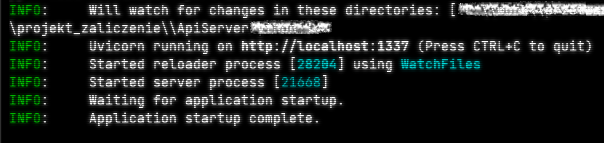
\includegraphics[width=0.8\textwidth]{assets/python_server_start.png}
        \caption{Ekran po uruchomieniu serwera Python}
        \label{fig:python_server_start}
    \end{figure}

    \begin{figure}[ht]
        \centering
        \noindent\hspace*{-1.8cm} % Dostosuj wartość -2.1cm według potrzeb
        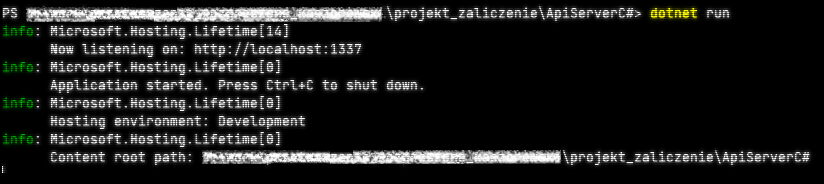
\includegraphics[width=1.0\textwidth]{assets/csharp_server_start.png}
        \caption{Ekran po uruchomieniu serwera C\#}
        \label{fig:csharp_server_start}
    \end{figure}
\end{spacing} % Kończymy interlinię 1.5

\subsection{Logowanie na serwerach Rest API}
\begin{spacing}{1.5} % Zaczynamy interlinię 1.5
    Na poniższym przykładzie na zdjęciach możemy zauważyć, że oba serwery logują poprawnie dane w swoim okienku terminala.. O ile terminal C\# zostawia więcej informacji tworzących szum o tyle wszystkie informacje potrzebne tam się znajdują.

    \begin{figure}[ht]
        \centering
        \noindent\hspace*{-2.1cm} % Dostosuj wartość -2.1cm według potrzeb
        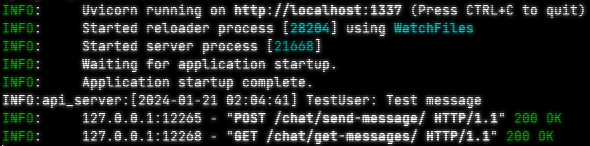
\includegraphics[width=1.2\textwidth]{assets/python_server_loging.png}
        \caption{Ekran logowań serwera Python}
        \label{fig:python_server_loging}
    \end{figure}


    \begin{figure}[ht]
        \centering
        \noindent\hspace*{-2.1cm} % Dostosuj wartość -2.1cm według potrzeb
        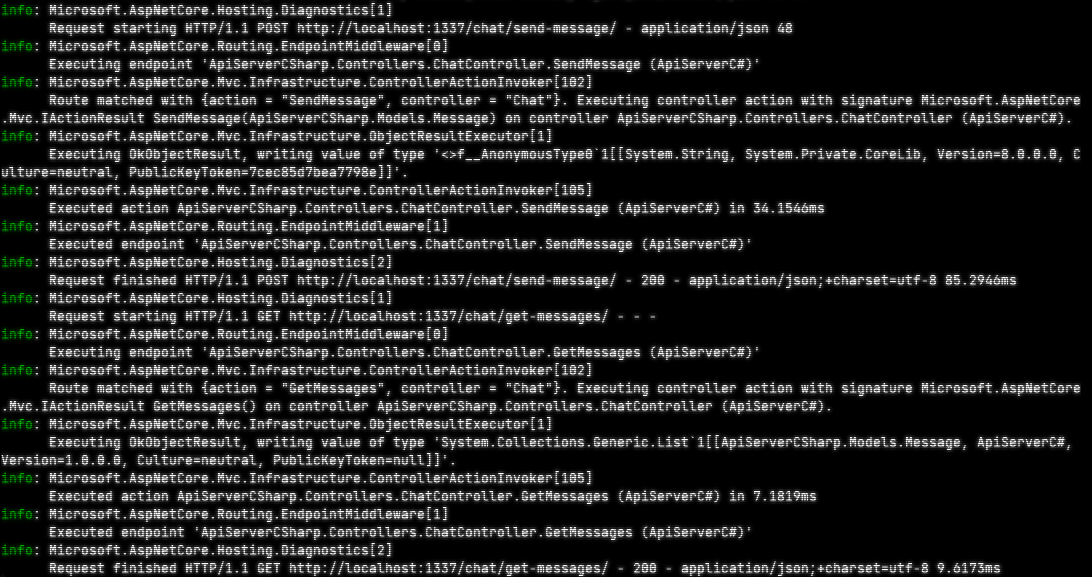
\includegraphics[width=1.2\textwidth]{assets/csharp_server_loging.png}
        \caption{Ekran logowań serwera C\#}
        \label{fig:csharp_server_loging}
    \end{figure}
\end{spacing} % Kończymy interlinię 1.5

\section{Używanie klienta REST API}
\subsection{Ekran powitalny}
\begin{spacing}{1.5} % Zaczynamy interlinię 1.5
    Użytkownik po uruchomieniu klienta chatu i jest przywitany komunikatem "Welcome to the Chat Client!".
    "Enter your username:" gdzie jest proszony o wpisanie nazwy użytkownika jaką będzie się posługiwał
    \begin{figure}[ht]
        \centering
        \noindent\hspace*{-2.1cm} % Dostosuj wartość -2.1cm według potrzeb
        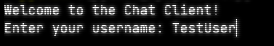
\includegraphics[width=1.2\textwidth]{assets/client_start.png}
        \caption{Ekran powitalny klienta REST API}
        \label{fig:client_start}
    \end{figure}
\end{spacing} % Kończymy interlinię 1.5

\subsection{Ekran menu}
\begin{spacing}{1.5} % Zaczynamy interlinię 1.5
    Po wprowadzeniu nazwy użytkownika, użytkownik widzi główne menu z opcjami. Opcje do wyboru to "Send a message", "Get message history" i "Exit".
    \begin{figure}[ht]
        \centering
        \noindent\hspace*{-2.1cm} % Dostosuj wartość -2.1cm według potrzeb
        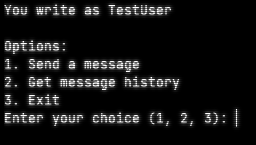
\includegraphics[width=1.0\textwidth]{assets/client_menu.png}
        \caption{Ekran menu klienta REST API}
        \label{fig:client_menu}
    \end{figure}
\end{spacing} % Kończymy interlinię 1.5

\subsection{Ekran wysyłania wiadomości}
\begin{spacing}{1.5} % Zaczynamy interlinię 1.5
\end{spacing} % Kończymy interlinię 1.5
    W oknie wysyłania wiadomości, użytkownik zostanie poproszony o wprowadzenie treści wiadomości. 
    \begin{figure}[ht]
        \centering
        \noindent\hspace*{-2.1cm} % Dostosuj wartość -2.1cm według potrzeb
        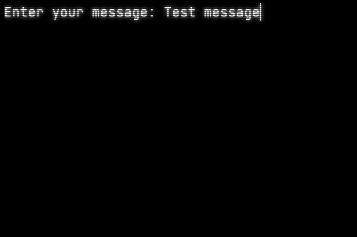
\includegraphics[width=0.8\textwidth]{assets/client_message.png}
        \caption{Ekran wysyłania wiadomości klienta REST API}
        \label{fig:client_message}
    \end{figure}

\subsection{Ekran po wysyłaniu wiadomości}
\begin{spacing}{1.5} % Zaczynamy interlinię 1.5
    Po wpisaniu i wysłaniu wiadomości, użytkownik otrzymuje potwierdzenie "Message sent successfully"
        \begin{figure}[ht]
        \centering
        \noindent\hspace*{-2.1cm} % Dostosuj wartość -2.1cm według potrzeb
        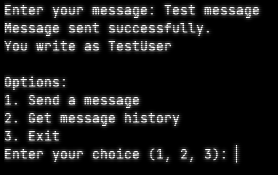
\includegraphics[width=0.8\textwidth]{assets/client_after_message.png}
        \caption{Ekran po wysyłaniu wiadomości klienta REST API}
        \label{fig:client_after_message}
    \end{figure}
\end{spacing} % Kończymy interlinię 1.5

\subsection{Ekran odczytywania wiadomości}
\begin{spacing}{1.5} % Zaczynamy interlinię 1.5
    Gdy użytkownik wybierze "Get message history", na ekranie wyświetlona zostanie historia wcześniej wysłanych wiadomości. Każda wiadomość jest wyświetlana wraz z nazwą użytkownika i treścią.
    \begin{figure}[ht]
        \centering
        \noindent\hspace*{-2.1cm} % Dostosuj wartość -2.1cm według potrzeb
        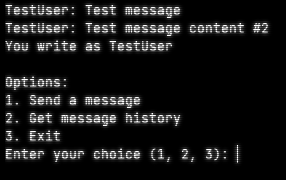
\includegraphics[width=0.6\textwidth]{assets/client_get.png}
        \caption{Ekran odczytywania wiadomości klienta REST API}
        \label{fig:client_get}
    \end{figure}
\end{spacing} % Kończymy interlinię 1.5

\subsection{Obsługa błędnego wyboru}
\begin{spacing}{1.5} % Zaczynamy interlinię 1.5
    W każdym momencie, jeśli użytkownik wprowadzi nieprawidłową opcję, system wyświetli komunikat "Invalid choice. Please enter 1, 2, or 3.", co zmusza użytkownika do podjęcia ponownej próby wyboru.
    \begin{figure}[ht]
        \centering
        \noindent\hspace*{-2.1cm} % Dostosuj wartość -2.1cm według potrzeb
        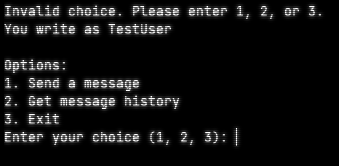
\includegraphics[width=0.6\textwidth]{assets/client_invalid_choice.png}
        \caption{Ekran obsługi błędnego wyboru klienta REST API}
        \label{fig:client_invalid_choice}
    \end{figure}
\end{spacing} % Kończymy interlinię 1.5

\subsection{Zakończenie sesji}
\begin{spacing}{1.5} % Zaczynamy interlinię 1.5
    Jeśli użytkownik zdecyduje się wyjść, wybierając "Exit", klient chatu zakończy działanie, informując użytkownika komunikatem "Exiting chat client.", co można zaobserwować po wykonaniu tej czynności
\end{spacing} % Kończymy interlinię 1.5

\section{Zakończenie}

\subsection{Czego się nauczyłem}
\begin{spacing}{1.5} % Zaczynamy interlinię 1.5
    Bardzo się cieszę, że mogłem poznać na zajęciach bibliotekę SignalR w związku z tym, że moja kariera zawodowa związana jest z warstwą sieciową internetu to jednak nie widzę przyszłości gdzie będę korzystał z tej biblioteki podczas gdy rynek oferuje o wiele prostsze rozwiązania oparte na api REST, SOAP, WebSocket i inne które można błyskawicznie zastosować.
\end{spacing} % Kończymy interlinię 1.5

\subsection{O projekcie}
\begin{spacing}{1.5} % Zaczynamy interlinię 1.5
    Powyższy projekt uważam za ciekawy choć przyznaję, że wybrałem projekt czatu gdyż taki projekt był wykonywany podczas zajęć. Zastanawiałem się nad projektem dokonującym autoryzacji lub innym command\&controll jednakże ostatecznie uznałem, że nie powinienem eksperymentować na zaliczenie, a ambitne projekty zostawić sobie na githuba.
\end{spacing} % Kończymy interlinię 1.5

\subsection{O ćwiczeniach}
\begin{spacing}{1.5} % Zaczynamy interlinię 1.5
    Jeśli chodzi o ćwiczenia to nie mam nic do zarzucenia prowadzącemu. Trochę żałuję, że zajęcia nie przystawały w moim mniemaniu do nazwy "przetwarzanie rozproszone" gdyż to sugeruje bardziej chmurowe kwestie aczkolwiek to nie jest problem. Zadaniem uczelni jest pokazać horyzonty, a to już w kwestii samego studenta jest to aby obrać kierunek w którym dalej będzie się specjalizował.
\end{spacing} % Kończymy interlinię 1.5